\section{Công trình liên quan}
Trong các hệ thống server và cloud hiện đại, dữ liệu giám sát thường được thu thập dưới dạng chuỗi thời gian từ nhiều lớp hạ tầng khác nhau, bao gồm máy chủ vật lý, máy ảo, container, microservice, cơ sở dữ liệu và hệ thống mạng. Các chỉ số như \textit{CPU utilization}, \textit{memory usage}, \textit{disk throughput}, \textit{network traffic}, \textit{request latency}, \textit{throughput} và \textit{error rate} phản ánh trạng thái vận hành của hệ thống theo thời gian. Do đó, phát hiện bất thường trên chuỗi thời gian đã trở thành một hướng nghiên cứu quan trọng nhằm phát hiện sớm các hiện tượng như quá tải tài nguyên, nghẽn cổ chai I/O, suy giảm hiệu năng dịch vụ, lỗi triển khai hoặc mất ổn định trong cụm cloud.

Chương này khảo sát ba nhóm công trình liên quan theo thứ tự xây dựng lập luận cho đề tài: các phương pháp phát hiện bất thường trên metric, các nghiên cứu ứng dụng LLM vào phân tích log và chẩn đoán nguyên nhân gốc rễ và các kiến trúc kết hợp hai hướng trên và cuối cùng  tổng kết khoảng trống nghiên cứu và định hướng thực nghiệm của đề tài.

Các công trình trong nhóm này có điểm chung là mô hình hóa hành vi bình thường của dữ liệu định lượng, sau đó xác định bất thường dựa trên mức độ sai lệch của quan sát mới so với mẫu hành vi đã học. Tuy nhiên, giữa các công trình vẫn có sự khác biệt rõ rệt về cách tiếp cận: một số nghiên cứu ưu tiên tính đơn giản và khả năng xử lý online, trong khi các nghiên cứu khác tập trung vào học quan hệ đa biến hoặc phụ thuộc dài hạn trong dữ liệu. Các hướng tiếp cận này là nền tảng quan trọng cho hệ thống giám sát thời gian thực, đồng thời cũng cho thấy giới hạn của việc chỉ dựa vào metric mà thiếu thông tin ngữ cảnh vận hành.
\subsection{Các nghiên cứu phát hiện bất thường trên chuỗi thời gian bằng mô hình thống kê và học sâu}
\subsection*{Công trình “Robust Random Cut Forest Based Anomaly Detection on Streams” của Guha và cộng sự}
Một hướng tiếp cận khác với các mô hình dự báo thống kê như ARIMA là phát hiện bất thường trực tiếp trên dòng dữ liệu bằng các cấu trúc cây ngẫu nhiên. Công trình \textbf{“Robust Random Cut Forest Based Anomaly Detection on Streams”} của Guha và cộng sự là một nghiên cứu tiêu biểu theo hướng này. Thay vì giả định chuỗi thời gian tuân theo một dạng mô hình tuyến tính hoặc mùa vụ cố định, công trình tập trung vào bài toán phát hiện bất thường trong dynamic data streams, nơi dữ liệu đến liên tục và mô hình phải được cập nhật nhanh khi có quan sát mới.

Ý tưởng trung tâm của công trình là sử dụng tập hợp các cây cắt ngẫu nhiên để duy trì một bản tóm tắt của dòng dữ liệu. Khi một điểm dữ liệu mới xuất hiện, hệ thống đánh giá mức độ “khác thường” của điểm đó dựa trên ảnh hưởng mà nó gây ra đối với cấu trúc dữ liệu hiện có. Nếu một điểm nằm ở vùng thưa, khác biệt rõ so với phần lớn quan sát trước đó, nó thường dễ bị cô lập trong cây và được gán điểm bất thường cao. Cách tiếp cận này kế thừa trực giác của các phương pháp cô lập bất thường, nhưng được thiết kế phù hợp hơn với dữ liệu luồng vì cấu trúc cây có thể được cập nhật khi dữ liệu mới đến.

Giá trị của công trình này đối với giám sát server/cloud nằm ở tính nhẹ và khả năng xử lý trực tuyến. Trong hạ tầng cloud, các metric như CPU utilization, memory usage, Disk I/O, network throughput, request latency hoặc error rate được sinh ra liên tục từ nhiều nguồn khác nhau. Một thuật toán như Robust Random Cut Forest có thể đóng vai trò là tầng phát hiện sơ cấp, nhanh chóng gắn điểm bất thường cho các quan sát mới mà không đòi hỏi quá trình huấn luyện nặng như nhiều mô hình học sâu. Đây cũng là lý do Random Cut Forest được triển khai trong các nền tảng cloud thực tế như Amazon SageMaker cho bài toán anomaly detection không giám sát.

So với \textbf{ARIMA}, hướng tiếp cận này linh hoạt hơn trong môi trường đa chiều. \textbf{ARIMA} thường phù hợp với từng chuỗi thời gian đơn biến và phụ thuộc nhiều vào đặc tính dự báo của chuỗi, trong khi \textbf{Random Cut Forest} có thể làm việc với dữ liệu nhiều chiều và không yêu cầu giả định mạnh về phân phối dữ liệu. Điều này hữu ích trong giám sát cloud, nơi một trạng thái hệ thống thường được mô tả đồng thời bởi nhiều metric, chẳng hạn CPU, RAM, network, số lượng request và độ trễ phản hồi.

Mặt khác, hạn chế của công trình vẫn nằm ở việc thuật toán chủ yếu đánh giá bất thường dựa trên hình dạng phân bố dữ liệu. Mô hình có thể xác định một điểm dữ liệu là khác biệt so với các quan sát trước đó, nhưng không tự biết sự khác biệt đó có ý nghĩa vận hành như thế nào. Trong cloud, một điểm có anomaly score cao có thể là dấu hiệu của sự cố, nhưng cũng có thể đến từ một hoạt động hợp lệ như batch job, backup định kỳ, rolling deployment, autoscaling hoặc migration dữ liệu. Vì vậy, \textbf{Robust Random Cut Forest} phù hợp để phát hiện nhanh các ứng viên bất thường, nhưng chưa đủ để quyết định cảnh báo cuối cùng nếu thiếu thông tin từ log, lịch vận hành và ngữ cảnh hệ thống.

\subsection*{Công trình “Multivariate Time-Series Anomaly Detection via Graph Attention Network” của Zhao và cộng sự}

\textbf{MTAD-GAT} của Zhao và cộng sự chuyển trọng tâm từ phát hiện bất thường đơn biến sang đa biến. Đây là bước tiến quan trọng trong giám sát hạ tầng cloud, nơi các chỉ số vận hành (như CPU, bộ nhớ, network) thường có mối tương quan chặt chẽ, và việc phân tích đơn lẻ dễ bỏ sót các bất thường phát sinh từ sự mất cân bằng giữa các metric.

Mô hình sử dụng cơ chế graph attention để học đồng thời mối quan hệ không gian giữa các biến và phụ thuộc thời gian. Bằng cách kết hợp hai nhiệm vụ dự báo và tái tạo chuỗi thời gian, \textbf{MTAD-GAT} tạo ra tín hiệu bất thường chính xác hơn, đồng thời giúp xác định các biến hoặc thời điểm có trọng số ảnh hưởng lớn nhất đến kết quả phát hiện.

Trong bối cảnh cloud, ưu điểm nổi bật của \textbf{MTAD-GAT} là khả năng phát hiện các bất thường dựa trên mối quan hệ giữa các chỉ số thay vì chỉ dựa trên ngưỡng tĩnh. Ví dụ, mô hình có thể phân biệt được việc CPU tăng cao là do tải thực sự hay do lỗi hệ thống dựa trên sự tương quan bất thường với các metric khác (như request rate hay memory), điều mà các phương pháp đơn biến truyền thống khó xử lý.

Tuy nhiên, \textbf{MTAD-GAT} chỉ học từ dữ liệu số nên chưa thể phân biệt nguyên nhân bất thường là do sự cố hay các hoạt động vận hành hợp lệ (như autoscaling, rolling update). Nếu thiếu thông tin ngữ cảnh từ log hoặc lịch triển khai, mô hình vẫn có nguy cơ tạo cảnh báo giả. Do đó, dù xử lý tốt bài toán tương quan đa biến, công trình này vẫn chưa lấp đầy khoảng trống về ngữ nghĩa trong giám sát hệ thống.

\subsection*{Công trình “Graph Neural Network-Based Anomaly Detection in Multivariate Time Series” của Deng và Hooi}

Deng và Hooi đề xuất mô hình \textbf{Graph Deviation Network (GDN)} nhằm học cấu trúc phụ thuộc giữa các biến trong chuỗi thời gian đa biến. Trong mô hình này, mỗi biến là một nút và các cạnh thể hiện mối quan hệ được học tự động từ dữ liệu, thay vì phải xây dựng đồ thị thủ công dựa trên kiến thức chuyên gia. GDN sử dụng thông tin từ các nút lân cận để dự đoán hành vi kỳ vọng của từng biến; nếu giá trị thực tế lệch đáng kể so với dự đoán, hệ thống sẽ ghi nhận bất thường. Ưu điểm chính của phương pháp này là không chỉ phát hiện độ lệch mà còn hỗ trợ thu hẹp phạm vi nguyên nhân thông qua việc phân tích trọng số của các cạnh trong đồ thị.

\textbf{Nhận xét chung về các mô hình dựa trên Graph (MTAD-GAT và GDN):} 
Cả hai công trình đều vượt trội so với phương pháp đơn biến nhờ khả năng tự học mối tương quan giữa các metric, giúp thu hẹp phạm vi phân tích nguyên nhân trong các hạ tầng cloud-native phức tạp. Tuy nhiên, điểm chung và cũng là giới hạn lớn nhất của chúng là chỉ dừng lại ở phân tích định lượng: mô hình có thể phát hiện sự mất cân bằng giữa các chỉ số, nhưng không thể tự phân biệt đâu là sự cố thực sự và đâu là hoạt động vận hành hợp lệ (như autoscaling, rolling update hay rebalancing). Do đó, để giảm thiểu cảnh báo giả và khép kín vòng lặp giám sát, các mô hình đồ thị này vẫn cần được tích hợp với một tầng phân tích ngữ cảnh từ log hoặc sự kiện hệ thống.

\subsection*{Nhận xét chung về nhóm công trình phát hiện bất thường chuỗi thời gian}

Ba công trình trên cho thấy ba hướng tiếp cận tiêu biểu trong phát hiện bất thường chuỗi thời gian cho hệ thống kỹ thuật và hạ tầng cloud.\textbf{ Robust Random Cut Forest} ưu tiên khả năng cập nhật nhanh và phát hiện bất thường trên dữ liệu luồng, phù hợp với vai trò bộ lọc sơ cấp. \textbf{MTAD-GAT} mở rộng bài toán sang chuỗi thời gian đa biến bằng cách học đồng thời quan hệ theo thời gian và theo đặc trưng. \textbf{Graph Deviation Network} tiếp tục đi sâu vào việc học cấu trúc quan hệ giữa các biến và hỗ trợ giải thích bất thường thông qua đồ thị và attention.

Điểm mạnh chung của các công trình này là khả năng xử lý dữ liệu định lượng với hiệu quả cao. Đây là yêu cầu quan trọng trong môi trường server/cloud, nơi metric được sinh ra liên tục và hệ thống giám sát cần phát hiện sớm các dấu hiệu bất thường. Các mô hình này có thể được sử dụng như tầng phát hiện ban đầu để sàng lọc dữ liệu bình thường, phát hiện các ứng viên bất thường và giảm tải cho các thành phần phân tích phía sau.

Hạn chế chung của nhóm phương pháp này là chúng vẫn phụ thuộc chủ yếu vào metric. Một bất thường về mặt số liệu không phải lúc nào cũng tương ứng với một sự cố cần cảnh báo. CPU tăng, Disk I/O tăng hoặc latency biến động có thể là dấu hiệu của lỗi hệ thống, nhưng cũng có thể là kết quả của các hoạt động hợp lệ như batch job, backup, rolling deployment, autoscaling, failover hoặc migration dữ liệu. Nếu không có thêm thông tin từ log, lịch vận hành, lịch triển khai hoặc tri thức hệ thống, các mô hình này khó phân biệt giữa bất thường thật sự và biến động hợp lệ.

Từ đó có thể thấy, các phương pháp phát hiện bất thường chuỗi thời gian vẫn giữ vai trò rất quan trọng trong kiến trúc giám sát thời gian thực nhờ tốc độ và khả năng xử lý dữ liệu lớn. Tuy nhiên, chúng phù hợp hơn với vai trò tầng phát hiện sơ cấp, thay vì là thành phần đưa ra quyết định cảnh báo cuối cùng. Để giảm cảnh báo giả và nâng cao chất lượng chẩn đoán, hệ thống cần một tầng phân tích bổ sung có khả năng liên kết metric với log, sự kiện vận hành và tri thức ngữ cảnh. Đây chính là tiền đề để khảo sát các nghiên cứu ứng dụng Mô hình Ngôn ngữ Lớn trong phân tích log, chẩn đoán nguyên nhân gốc rễ và suy luận ngữ cảnh ở phần tiếp theo.
\subsection{Các nghiên cứu ứng dụng LLM trong phân tích log và chẩn đoán nguyên nhân gốc rễ}

Bên cạnh dữ liệu metric dạng chuỗi thời gian, log hệ thống là một nguồn thông tin quan trọng trong quá trình vận hành server và cloud. Nếu metric phản ánh trạng thái định lượng của hệ thống, chẳng hạn CPU, RAM, Disk I/O, latency hoặc error rate, thì log lại chứa thông tin mô tả sự kiện, trạng thái tiến trình, lỗi ứng dụng, truy vấn cơ sở dữ liệu, thao tác triển khai và các thông báo từ hệ điều hành hoặc middleware. Do đó, log thường được sử dụng trong các tác vụ như log parsing, phát hiện bất thường dựa trên log, phân tích sự cố và chẩn đoán nguyên nhân gốc rễ.

Trước khi Mô hình Ngôn ngữ Lớn được ứng dụng rộng rãi, nhiều phương pháp phân tích log dựa vào biểu thức chính quy, luật thủ công, clustering hoặc mô hình học máy truyền thống. Tuy nhiên, log trong các hệ thống cloud hiện đại thường có cấu trúc đa dạng, thay đổi liên tục theo phiên bản phần mềm và chứa nhiều thông tin bán cấu trúc hoặc phi cấu trúc. Đây là lý do các nghiên cứu gần đây bắt đầu khai thác LLM để tận dụng khả năng hiểu ngôn ngữ tự nhiên, hiểu mã nguồn, nhận diện mẫu văn bản kỹ thuật và liên kết nhiều nguồn thông tin khác nhau trong quá trình phân tích vận hành.

\subsection*{Công trình “LogParser-LLM: Advancing Efficient Log Parsing with Large Language Models” của Zhong và cộng sự}

\textbf{Log parsing} là bước nền tảng trong nhiều hệ thống phân tích log, vì nó chuyển đổi các dòng log thô thành các template có cấu trúc để phục vụ các tác vụ phía sau như phát hiện bất thường, phân tích lỗi hoặc tìm nguyên nhân gốc rễ. Công trình LogParser-LLM của Zhong và cộng sự tập trung vào vấn đề này bằng cách tích hợp khả năng ngữ nghĩa của LLM vào quá trình log parsing. Khác với nhiều phương pháp truyền thống cần tinh chỉnh siêu tham số hoặc phụ thuộc vào dữ liệu huấn luyện có nhãn,\textbf{ LogParser-LLM} hướng đến khả năng thích nghi nhanh với log mới và môi trường hệ thống thay đổi.

Điểm đáng chú ý của công trình là tác giả không chỉ sử dụng LLM một cách trực tiếp cho từng dòng log, mà còn quan tâm đến hiệu quả triển khai. Trong đánh giá trên LogPub, một benchmark log quy mô lớn với trung bình khoảng 3,6 triệu dòng log trên mỗi tập dữ liệu thuộc 14 hệ thống, \textbf{LogParser-LLM} chỉ cần trung bình 272,5 lần gọi LLM, đồng thời đạt 90,6\% F1 cho grouping accuracy và 81,1\% cho parsing accuracy. Kết quả này cho thấy LLM có thể hỗ trợ log parsing hiệu quả nếu được thiết kế theo hướng tiết kiệm số lần gọi mô hình, thay vì đưa toàn bộ log thô vào LLM một cách trực tiếp.

Đối với bài toán giám sát server/cloud, công trình này có ý nghĩa quan trọng vì log parsing là bước tiền xử lý cần thiết để biến log phi cấu trúc thành thông tin có thể liên kết với metric. Ví dụ, khi hệ thống ghi nhận latency tăng hoặc CPU tăng bất thường, các template log liên quan đến deployment, timeout, database connection hoặc cache miss có thể cung cấp ngữ cảnh cần thiết để giải thích biến động metric. Nhờ khả năng hiểu ngữ nghĩa của log, LLM có thể xử lý tốt hơn các mẫu log phức tạp hoặc thay đổi theo phiên bản phần mềm.

Mặt khác, \textbf{LogParser-LLM} vẫn chủ yếu giải quyết bài toán chuyển đổi log thô thành template có cấu trúc. Công trình này chưa trực tiếp giải quyết việc ra quyết định cảnh báo trong một pipeline giám sát thời gian thực. Ngoài ra, dù số lần gọi LLM đã được tối ưu, việc sử dụng LLM trong log parsing vẫn đặt ra các vấn đề về chi phí, độ trễ và tính ổn định đầu ra khi áp dụng vào hệ thống có lượng log rất lớn. Do đó, hướng tiếp cận này phù hợp để tăng chất lượng dữ liệu log đầu vào, nhưng cần được kết hợp với các tầng xử lý khác nếu muốn sử dụng trong giám sát online.

\subsection*{Công trình “LogLLM: Log-based Anomaly Detection Using Large Language Models” của Guan và cộng sự}

Nếu \textbf{LogParser-LLM} tập trung vào bước parsing, thì \textbf{LogLLM} của Guan và cộng sự đi xa hơn khi sử dụng LLM cho bài toán phát hiện bất thường dựa trên log. Công trình này xuất phát từ nhận định rằng log chứa nhiều thông tin ngữ nghĩa dưới dạng ngôn ngữ tự nhiên, trong khi các phương pháp học sâu truyền thống thường gặp khó khăn trong việc khai thác đầy đủ ý nghĩa của các thông điệp log. Vì vậy, nhóm tác giả đề xuất một framework sử dụng BERT để trích xuất vector ngữ nghĩa từ log message, sau đó dùng Llama làm mô hình phân loại chuỗi log.

Bên cạnh đó, \textbf{LogLLM} là công trình không phụ thuộc hoàn toàn vào log parser truyền thống để trích xuất template. Thay vào đó, hệ thống tiền xử lý log bằng biểu thức chính quy và khai thác biểu diễn ngữ nghĩa từ mô hình ngôn ngữ. Đồng thời, nhóm tác giả sử dụng một projector để căn chỉnh không gian biểu diễn giữa BERT và Llama, giúp mô hình phân loại hiểu tốt hơn các đặc trưng ngữ nghĩa được trích xuất. Cách thiết kế này cho thấy LLM không chỉ được dùng như một chatbot trả lời câu hỏi, mà có thể được tích hợp vào pipeline học máy cho log anomaly detection.

Kết quả thực nghiệm của \textbf{LogLLM} trên bốn bộ dữ liệu log công khai cho thấy framework này vượt qua các phương pháp hiện đại trước đó, đặc biệt trong bối cảnh log không ổn định. Đây là điểm quan trọng đối với hệ thống cloud, nơi log có thể thay đổi sau mỗi lần cập nhật ứng dụng, thay đổi dependency hoặc thay đổi cấu hình hạ tầng. Khả năng nắm bắt ý nghĩa của thông điệp log giúp LLM phân biệt tốt hơn giữa các mẫu log bình thường và các chuỗi log phản ánh lỗi hệ thống.

Tuy nhiên, hạn chế của \textbf{LogLLM} là nó vẫn chủ yếu vận hành trên dữ liệu log, trong khi sự cố cloud thường cần được phân tích từ nhiều nguồn telemetry khác nhau, bao gồm metric, trace, sự kiện triển khai và tài liệu vận hành. Ngoài ra, việc sử dụng BERT, Llama và quá trình huấn luyện nhiều giai đoạn có thể tạo ra chi phí tính toán đáng kể. Điều này khiến \textbf{LogLLM} phù hợp với bài toán log anomaly detection có kiểm soát, nhưng chưa hẳn phù hợp để xử lý trực tiếp toàn bộ log stream tốc độ cao trong một hệ thống giám sát thời gian thực.

\subsection*{Công trình “RCAgent: Cloud Root Cause Analysis by Autonomous Agents with Tool-Augmented Large Language Models” của Wang và cộng sự}

Trong khi các công trình \textbf{log parsing} và \textbf{log anomaly detection} tập trung vào việc phát hiện dấu hiệu bất thường, bài toán \textbf{Root Cause Analysis} xác định nguyên nhân gốc rễ của sự cố. Công trình \textbf{RCAgent }của Wang và cộng sự là một nghiên cứu tiêu biểu ứng dụng LLM vào RCA trong môi trường cloud. Công trình này đề xuất một framework agent tự chủ, trong đó LLM không chỉ phân tích văn bản đầu vào mà còn được tăng cường bằng công cụ để tương tác với môi trường, truy vấn dữ liệu và thực hiện các bước điều tra có cấu trúc.

Điểm khác biệt của \textbf{RCAgent} nằm ở cách nhìn nhận LLM như một tác nhân điều tra sự cố, thay vì chỉ là một mô hình sinh câu trả lời. Trong quá trình RCA, agent có thể lập kế hoạch, chọn công cụ phù hợp, truy xuất thông tin liên quan và từng bước thu hẹp phạm vi nguyên nhân. Điều này phản ánh khá gần quy trình làm việc của kỹ sư vận hành cloud: khi một incident xảy ra, người vận hành thường phải kiểm tra metric, log, trace, dependency, lịch triển khai và các thay đổi gần thời điểm xảy ra lỗi. \textbf{RCAgent} cố gắng tự động hóa một phần quy trình đó bằng khả năng suy luận và ra quyết định của LLM.

Giá trị của \textbf{RCAgent} đối với lĩnh vực AIOps là nó cho thấy LLM có tiềm năng trong việc liên kết nhiều nguồn thông tin rời rạc để hỗ trợ chẩn đoán. Trong môi trường cloud, nguyên nhân của một sự cố không nhất thiết nằm ở metric bất thường rõ ràng nhất. Ví dụ, latency của API có thể tăng do database connection pool cạn kiệt, cache miss tăng, dependency bên ngoài chậm hoặc một bản triển khai mới làm thay đổi logic truy vấn. Một LLM agent có khả năng dùng công cụ có thể lần theo các dấu hiệu này và đưa ra giả thuyết nguyên nhân hợp lý hơn so với mô hình chỉ phân tích một loại dữ liệu.

Dù vậy, \textbf{RCAgent} chủ yếu phù hợp với giai đoạn điều tra sau khi sự cố hoặc cảnh báo đã xuất hiện. Quy trình agent thường bao gồm nhiều bước suy luận, nhiều lần truy xuất dữ liệu và nhiều lần gọi mô hình, nên khó đáp ứng yêu cầu độ trễ thấp nếu đặt trực tiếp trên đường đi của luồng giám sát thời gian thực. Ngoài ra, việc triển khai agent trong môi trường sản xuất còn gặp các thách thức về quyền truy cập dữ liệu, bảo mật, kiểm soát hành động của agent và chi phí vận hành. Vì vậy, RCAgent thể hiện năng lực mạnh của LLM trong RCA, nhưng vẫn chưa giải quyết trọn vẹn bài toán phát hiện và thẩm định cảnh báo ở tốc độ streaming.
\subsection*{Nhận xét chung về nhóm công trình ứng dụng LLM trong phân tích log và chẩn đoán nguyên nhân gốc rễ}
Ba công trình \textbf{LogParser-LLM}, \textbf{LogLLM} và \textbf{RCAgent} cho thấy LLM có thể được ứng dụng ở nhiều giai đoạn khác nhau trong quy trình vận hành hệ thống. LogParser-LLM tập trung vào việc chuyển đổi log thô thành cấu trúc có thể phân tích, LogLLM khai thác ngữ nghĩa của log để phát hiện bất thường, còn \textbf{RCAgent} sử dụng LLM như một tác nhân hỗ trợ điều tra và chẩn đoán nguyên nhân gốc rễ trong môi trường cloud.

Điểm mạnh chung của các công trình này là khả năng xử lý thông tin ngữ nghĩa mà các mô hình chuỗi thời gian truyền thống khó khai thác. Thông qua log, tài liệu vận hành, thông tin sự kiện và dữ liệu hệ thống, LLM có thể hỗ trợ liên kết các dấu hiệu rời rạc, diễn giải bối cảnh và đưa ra nhận định gần với cách kỹ sư vận hành phân tích sự cố.

Ngoài ra, các phương pháp này vẫn tồn tại hạn chế khi áp dụng vào giám sát thời gian thực. Việc gọi LLM thường có chi phí cao, độ trễ lớn và khó mở rộng nếu phải xử lý trực tiếp toàn bộ log hoặc metric stream. Ngoài ra, các hệ thống như RCAgent thường phù hợp hơn với giai đoạn sau khi sự cố đã xảy ra, thay vì phát hiện và thẩm định cảnh báo ngay trong luồng dữ liệu.

\subsection{Các kiến trúc giám sát lai và cơ chế đánh giá LLM-as-a-Judge}
Các công trình ở mục 3.1 cho thấy các mô hình chuỗi thời gian có khả năng xử lý nhanh dữ liệu metric, nhưng còn hạn chế trong việc hiểu ngữ cảnh vận hành. Ngược lại, các công trình ở mục 3.2 cho thấy LLM có khả năng phân tích log, tổng hợp thông tin và hỗ trợ chẩn đoán nguyên nhân gốc rễ, nhưng lại gặp vấn đề về chi phí và độ trễ nếu sử dụng trực tiếp trên toàn bộ dữ liệu giám sát. Từ hai hướng tiếp cận này, một xu hướng nghiên cứu mới đã hình thành: xây dựng các kiến trúc lai, trong đó mô hình nhỏ hoặc mô hình chuyên biệt đảm nhiệm việc phát hiện ban đầu, còn LLM được sử dụng ở tầng sau để giải thích, thẩm định hoặc bổ sung ngữ cảnh.

Điểm cốt lõi của kiến trúc lai là không xem LLM như bộ quét chính trên toàn bộ luồng dữ liệu. Thay vào đó, LLM chỉ xử lý các sự kiện đã được chọn lọc, chẳng hạn các điểm bất thường, cảnh báo nghi vấn hoặc đoạn dữ liệu cần giải thích. Cách tiếp cận này giúp tận dụng khả năng suy luận ngữ nghĩa của LLM, đồng thời hạn chế số lần gọi mô hình, giảm chi phí token và giảm độ trễ đầu cuối. Trong nhóm nghiên cứu này, các công trình tiêu biểu có thể kể đến RAAD-LLM, ARGOS, CALM và nghiên cứu về "LLM-as-a-Judge for Time Series Explanations".

\subsection*{Công trình “RAAD-LLM: Adaptive Anomaly Detection Using LLMs and RAG Integration” của Russell-Gilbert và cộng sự}

Công trình \textbf{RAAD-LLM} của Russell-Gilbert và cộng sự khai thác LLM kết hợp với Retrieval-Augmented Generation để giải quyết bài toán phát hiện bất thường thích ứng trong môi trường công nghiệp. Bối cảnh chính của công trình là predictive maintenance, nơi dữ liệu vận hành thường thưa, điều kiện hoạt động thay đổi và tri thức miền đóng vai trò quan trọng trong quá trình đánh giá bất thường. Thay vì chỉ dựa vào dữ liệu chuỗi thời gian, RAAD-LLM bổ sung tri thức liên quan thông qua cơ chế truy xuất, sau đó cung cấp thông tin này cho LLM để hỗ trợ quá trình phân tích. Công trình báo cáo độ chính xác trên dữ liệu thực tế tăng từ 70,7\% lên 88,6\% so với mô hình trước đó của nhóm tác giả.

Ý nghĩa chính của \textbf{RAAD-LLM} nằm ở việc đưa tri thức ngữ cảnh vào quá trình phát hiện bất thường. Trong nhiều hệ thống thực tế, một biến động dữ liệu không thể được đánh giá chỉ bằng giá trị số. Cần có thêm thông tin về chế độ vận hành, lịch bảo trì, loại thiết bị, điều kiện môi trường hoặc kinh nghiệm chuyên gia. RAG giúp LLM truy xuất các thông tin liên quan thay vì chỉ dựa vào kiến thức có sẵn trong mô hình. Nhờ đó, hệ thống có thể đưa ra nhận định phù hợp hơn với bối cảnh cụ thể của từng sự kiện.

Đối với bài toán giám sát server/cloud, hướng tiếp cận của \textbf{RAAD-LLM} gợi ý rằng LLM nên được cung cấp thêm log, lịch triển khai, tài liệu vận hành hoặc các sự kiện hệ thống trước khi đưa ra đánh giá. Ví dụ, một đợt tăng Disk I/O có thể được xem là bất thường nếu không có ngữ cảnh, nhưng sẽ hợp lý nếu RAG truy xuất được thông tin rằng hệ thống đang thực hiện backup định kỳ. Tuy nhiên, RAAD-LLM chủ yếu được kiểm chứng trong bối cảnh bảo trì dự đoán công nghiệp, chưa tập trung trực tiếp vào pipeline giám sát cloud có yêu cầu xử lý luồng dữ liệu liên tục và độ trễ thấp. Ngoài ra, việc truy xuất tri thức và gọi LLM vẫn tạo thêm chi phí, nên cần có cơ chế chọn lọc sự kiện đầu vào.

\subsection*{Công trình “ARGOS: Agentic Time-Series Anomaly Detection with Autonomous Rule Generation via Large Language Models” của Gu và cộng sự}

Khác với \textbf{RAAD-LLM}, công trình ARGOS không sử dụng LLM để trực tiếp đánh giá từng điểm dữ liệu bất thường. Thay vào đó, hệ thống dùng LLM để tự động sinh ra các luật phát hiện bất thường cho dữ liệu chuỗi thời gian trong hạ tầng cloud. Các luật này đóng vai trò như một biểu diễn trung gian: có thể giải thích được, có thể tái lập và có thể triển khai với chi phí thấp trong môi trường online. Đây là điểm rất quan trọng đối với các hệ thống sản xuất, nơi một cảnh báo không chỉ cần chính xác mà còn phải dễ kiểm tra và dễ bảo trì.

Trong \textbf{ARGOS}, LLM được đặt ở vai trò hỗ trợ xây dựng logic phát hiện thay vì thay thế hoàn toàn bộ phát hiện bất thường. Hệ thống sử dụng nhiều agent phối hợp để sinh, kiểm tra và huấn luyện các luật phát hiện. Sau khi luật được tạo và xác nhận, chúng có thể được triển khai để phát hiện bất thường với chi phí thấp hơn nhiều so với việc gọi LLM liên tục. Kết quả thực nghiệm cho thấy ARGOS cải thiện F1-score lên đến 9,5\% trên các tập dữ liệu công khai và 28,3\% trên tập dữ liệu nội bộ của Microsoft.

Giá trị của \textbf{ARGOS} đối với giám sát cloud nằm ở việc nó giải quyết ba yêu cầu quan trọng: khả năng giải thích, tính tái lập và tự động hóa. Trong thực tế, các mô hình học sâu có thể phát hiện bất thường tốt nhưng khó giải thích vì sao một điểm bị gắn cờ. Ngược lại, luật phát hiện có thể được con người kiểm tra, chỉnh sửa và triển khai dễ dàng hơn. Tuy nhiên, hướng tiếp cận này cũng có giới hạn. \textbf{ARGOS} phù hợp với việc tạo ra các luật phát hiện có thể chạy online, nhưng bản thân các luật vẫn chủ yếu dựa trên mẫu metric. Nếu một biến động hợp lệ chưa được phản ánh đúng trong luật hoặc thiếu thông tin ngữ cảnh từ log và lịch vận hành, hệ thống vẫn có thể tạo cảnh báo giả.

\subsection*{Công trình “CALM: A Framework for Continuous, Adaptive, and LLM-Mediated Anomaly Detection in Time-Series Streams” của Devireddy và Huang}

Công trình \textbf{CALM} là một trong những nghiên cứu gần nhất với hướng của đề tài vì đặt bài toán trong môi trường time-series streams và sử dụng LLM như một thành phần trung gian để hỗ trợ đánh giá bất thường. \textbf{CALM} được xây dựng như một framework phát hiện bất thường thời gian thực, sử dụng \textbf{Apache Beam} cho xử lý phân tán, \textbf{TimesFM} cho phát hiện bất thường dựa trên dự báo, và một thành phần \textbf{LLM-as-a-Judge} để đưa ra đánh giá ngữ nghĩa đối với các bất thường được phát hiện.

Điểm nổi bật của \textbf{CALM} là cơ chế thích ứng liên tục. Các mô hình phát hiện bất thường thường bị suy giảm hiệu năng khi dữ liệu thay đổi theo thời gian, tức gặp hiện tượng concept drift. \textbf{CALM} giải quyết vấn đề này bằng cách fine-tuning liên tục mô hình phát hiện, đồng thời dùng LLM-as-a-Judge để đánh giá xem một bất thường là nhiễu tạm thời hay là một thay đổi mẫu có ý nghĩa. Nhờ đó, hệ thống không chỉ phát hiện bất thường mà còn có khả năng cập nhật hiểu biết về trạng thái bình thường mới của dữ liệu. Kết quả đánh giá trên benchmark \textbf{TSB-UAD} cho thấy mô hình được fine-tuning liên tục cải thiện \textbf{ROC AUC} trên phần lớn tập dữ liệu so với mô hình nền tĩnh.

Đối với đề tài này, \textbf{CALM} có giá trị tham khảo trực tiếp vì thể hiện rõ nguyên tắc phân tầng: mô hình chuyên biệt xử lý luồng dữ liệu, còn LLM chỉ tham gia ở bước đánh giá và điều phối ngữ nghĩa. Đây cũng là cách tiếp cận phù hợp để hạn chế chi phí và độ trễ của LLM. Tuy nhiên, \textbf{CALM} tập trung nhiều vào cơ chế thích ứng và fine-tuning liên tục trên chuỗi thời gian không dừng, trong khi bài toán của đề tài nhấn mạnh thêm khía cạnh giảm cảnh báo giả bằng cách liên kết metric với log, lịch triển khai và ngữ cảnh vận hành trong hệ thống server/cloud. Vì vậy, \textbf{CALM} là công trình gần nhất về mặt kiến trúc, nhưng vẫn còn khoảng trống để mở rộng theo hướng thẩm định cảnh báo dựa trên nhiều nguồn telemetry.

\subsection*{Công trình “LLM-as-a-Judge for Time Series Explanations” của Sivalingam và cộng sự}

Một hướng nghiên cứu liên quan đến cơ chế đánh giá tự động là công trình \textbf{LLM-as-a-Judge for Time Series Explanations} của Sivalingam và cộng sự. Khác với các công trình tập trung vào phát hiện bất thường, nghiên cứu này khảo sát khả năng dùng LLM để đánh giá lời giải thích được sinh ra cho dữ liệu chuỗi thời gian. Công trình xây dựng một benchmark gồm 350 trường hợp chuỗi thời gian, bao phủ bảy loại truy vấn, trong đó mỗi trường hợp đi kèm các lời giải thích đúng, đúng một phần và sai.

Kết quả của công trình cho thấy LLM có thể hoạt động ổn định hơn khi đóng vai trò bộ đánh giá so với khi đóng vai trò bộ sinh lời giải thích. Nói cách khác, LLM không phải lúc nào cũng tự tạo ra phân tích chính xác, nhưng có thể tương đối hữu ích trong việc chấm điểm, xếp hạng hoặc phân biệt lời giải thích đúng và sai khi được cung cấp dữ liệu và tiêu chí đánh giá rõ ràng. Đây là một kết luận quan trọng đối với các hệ thống giám sát lai: LLM có thể phù hợp hơn khi được đặt ở vai trò thẩm định, kiểm tra hoặc đánh giá cảnh báo, thay vì tự mình quét toàn bộ dữ liệu và đưa ra kết luận từ đầu.

Đối với bài toán giám sát server/cloud, ý tưởng LLM-as-a-Judge có thể được mở rộng từ việc đánh giá lời giải thích sang đánh giá cảnh báo. Sau khi một mô hình phát hiện sơ cấp xác định một điểm hoặc một đoạn metric bất thường, LLM có thể nhận thêm log, sự kiện triển khai, lịch bảo trì và tài liệu vận hành để đánh giá liệu cảnh báo đó có đáng tin cậy hay không. Tuy nhiên, công trình này chủ yếu nghiên cứu trên benchmark tổng hợp về giải thích chuỗi thời gian, chưa trực tiếp triển khai trong một pipeline giám sát cloud thực tế. Do đó, nó cung cấp cơ sở lý luận cho vai trò “judge” của LLM, nhưng cần được kết hợp với kiến trúc streaming và dữ liệu vận hành thực tế để áp dụng vào hệ thống giám sát.

\subsubsection*{Công trình “Nezha: Interpretable Fine-Grained Root Causes Analysis for Microservices on Multi-modal Observability Data” của Yu và cộng sự}
Nezha đề xuất một framework chẩn đoán nguyên nhân gốc rễ phi giám sát
cho hệ thống microservice, với điểm khác biệt chính là phân tích hợp nhất
cả ba nguồn telemetry — metric, log và trace — thay vì chỉ dựa vào một
loại dữ liệu. Ý tưởng trung tâm là chuyển đổi các dữ liệu không đồng nhất
này thành một biểu diễn sự kiện thống nhất, sau đó xây dựng đồ thị sự kiện
cho từng request dựa trên trace ID và span ID. Bằng cách so sánh mẫu thực
thi giữa giai đoạn bình thường và giai đoạn xảy ra lỗi, hệ thống định vị
nguyên nhân ở mức chi tiết — cụ thể đến vùng mã nguồn hoặc loại tài nguyên
bị nghẽn. Trên 101 kịch bản tiêm lỗi với hai ứng dụng microservice chuẩn,
Nezha đạt độ chính xác Top-1 trung bình 89,77\%, vượt các phương pháp
tiên tiến trước đó từ 61,45\% đến 74,85\%.

Đối với đề tài này, Nezha có giá trị tham khảo ở hai khía cạnh. Thứ nhất,
hướng tiếp cận đa nguồn telemetry của công trình cho thấy việc kết hợp
metric với log và trace giúp khép kín khoảng trống thông tin mà các phương
pháp đơn nguồn bỏ sót — đây là tiền đề trực tiếp cho kiến trúc hai tầng
của đề tài. Thứ hai, bộ dữ liệu thực nghiệm mà nhóm tác giả mở mã nguồn
cung cấp một môi trường kiểm chứng lý tưởng với đầy đủ nhãn lỗi theo
fault type, service và pod, hỗ trợ đánh giá pipeline RAG và LLM-as-a-Judge
trong điều kiện gần với thực tế vận hành.

Hạn chế của Nezha nằm ở tính ngoại tuyến của quy trình xử lý. Việc xây
dựng đồ thị sự kiện và khai phá mẫu đòi hỏi năng lực tính toán đáng kể
và chu kỳ xử lý nhất định, khó đáp ứng yêu cầu độ trễ thấp của các hệ
thống cảnh báo streaming. Vì vậy, Nezha phù hợp hơn với vai trò tầng chẩn
đoán chuyên sâu sau khi sự cố đã được phát hiện, thay vì đặt trực tiếp trên
đường đi của luồng giám sát thời gian thực.


\subsection*{Nhận xét chung về nhóm kiến trúc giám sát lai}

Các công trình trên cho thấy xu hướng chung là không sử dụng LLM như một bộ phát hiện bất thường độc lập, mà đặt LLM vào một kiến trúc phân tầng. Trong RAAD-LLM, LLM được tăng cường bằng RAG để khai thác tri thức miền. Trong ARGOS, LLM được dùng để sinh luật phát hiện bất thường có thể triển khai online với chi phí thấp. Trong CALM, LLM đóng vai trò đánh giá ngữ nghĩa đối với các bất thường được phát hiện trong luồng chuỗi thời gian. Còn trong nghiên cứu LLM-as-a-Judge for Time Series Explanations, LLM được khảo sát như một bộ đánh giá tính đúng đắn của lời giải thích chuỗi thời gian.

Điểm mạnh của các kiến trúc này là khả năng dung hòa giữa tốc độ xử lý của các mô hình chuyên biệt và năng lực suy luận ngữ cảnh của LLM. Thay vì đưa toàn bộ metric hoặc log stream vào LLM, hệ thống có thể dùng mô hình nhẹ để sàng lọc trước, sau đó chỉ chuyển các sự kiện nghi vấn sang LLM để phân tích sâu. Cách tiếp cận này giúp giảm chi phí, giảm độ trễ và tăng khả năng mở rộng so với việc sử dụng LLM trực tiếp trên toàn bộ dữ liệu giám sát.

Tuy nhiên, các công trình hiện tại vẫn còn một số giới hạn. Một số nghiên cứu tập trung vào môi trường công nghiệp hoặc predictive maintenance, chưa trực tiếp xử lý bài toán giám sát server/cloud. Một số hướng khác tập trung vào sinh luật hoặc đánh giá lời giải thích, nhưng chưa đi sâu vào việc thẩm định cảnh báo bằng cách kết hợp đồng thời metric, log và sự kiện vận hành. Ngoài ra, chi phí gọi LLM, độ trễ suy luận và cách lựa chọn dữ liệu đầu vào vẫn là các vấn đề cần được kiểm soát chặt chẽ khi triển khai trong môi trường thời gian thực.


\subsection{Tổng kết khoảng trống nghiên cứu và định hướng của đề tài}

\begin{table}[h!]
    \centering
    \caption{Tổng hợp các nhóm công trình nghiên cứu liên quan}
    \label{tab:related-work-summary}
    \renewcommand{\arraystretch}{1.35}
    \setlength{\tabcolsep}{4pt}
    \small
    \begin{tabularx}{\textwidth}{|
        >{\raggedright\arraybackslash}p{2.7cm}|
        >{\raggedright\arraybackslash}p{3.0cm}|
        >{\raggedright\arraybackslash}p{2.8cm}|
        >{\raggedright\arraybackslash}X|
        >{\raggedright\arraybackslash}X|
    }
        \hline
        \textbf{Nhóm công trình} 
        & \textbf{Công trình tiêu biểu} 
        & \textbf{Vai trò chính} 
        & \textbf{Ưu điểm} 
        & \textbf{Hạn chế} \\
        \hline

        Phát hiện bất thường trên chuỗi thời gian
        & Robust Random Cut Forest, MTAD-GAT, Graph Deviation Network
        & Phát hiện bất thường từ metric
        & Xử lý nhanh, phù hợp dữ liệu luồng, khai thác được quan hệ đa biến
        & Thiếu khả năng hiểu ngữ cảnh vận hành, dễ sinh cảnh báo giả \\
        \hline

        LLM cho phân tích log
        & LogParser-LLM, LogLLM
        & Chuẩn hóa log và phát hiện bất thường từ log
        & Khai thác tốt thông tin ngữ nghĩa trong log
        & Chi phí cao nếu xử lý log quy mô lớn, chưa kết hợp đầy đủ metric và sự kiện vận hành \\
        \hline

        LLM cho RCA
        & RCAgent
        & Hỗ trợ điều tra và tìm nguyên nhân gốc rễ
        & Có khả năng lập luận, truy xuất thông tin và hỗ trợ kỹ sư vận hành
        & Thường hoạt động sau khi sự cố xảy ra, độ trễ cao, khó đặt trực tiếp vào pipeline thời gian thực \\
        \hline

        Kiến trúc lai và LLM-as-a-Judge
        & RAAD-LLM, ARGOS, CALM
        & Kết hợp mô hình nhỏ với LLM để đánh giá hoặc giải thích
        & Giảm tải cho LLM, tận dụng được ngữ cảnh, phù hợp hướng phân tầng
        & Vẫn cần kiểm soát chi phí, độ trễ và cách lựa chọn dữ liệu đưa vào LLM \\
        \hline
    \end{tabularx}
\end{table}
\subsection*{Khoảng trống nghiên cứu}
Từ các công trình đã khảo sát, có thể thấy mỗi hướng tiếp cận vẫn tồn tại những giới hạn riêng. Các mô hình phát hiện bất thường trên chuỗi thời gian như \textbf{Robust Random Cut Forest},\textbf{ MTAD-GAT} và \textbf{Graph Deviation Network} có ưu điểm về tốc độ xử lý và phù hợp với dữ liệu metric trong môi trường server/cloud. Tuy nhiên, các mô hình này chủ yếu dựa trên sự sai lệch định lượng nên khó phân biệt giữa sự cố thật sự và các biến động hợp lệ do batch job, backup định kỳ, autoscaling, rolling deployment hoặc migration dữ liệu.

Trong khi đó, các công trình ứng dụng LLM như \textbf{LogParser-LLM},\textbf{ LogLLM} và\textbf{ RCAgent} cho thấy khả năng khai thác thông tin ngữ nghĩa từ log, tài liệu vận hành và sự kiện hệ thống. Tuy nhiên, LLM thường có chi phí suy luận cao, độ trễ lớn và khó xử lý trực tiếp toàn bộ luồng metric/log trong thời gian thực. Nhiều hệ thống cũng thiên về phân tích sau khi sự cố đã xảy ra, thay vì thẩm định cảnh báo ngay trong quá trình giám sát.

Các kiến trúc như \textbf{RAAD-LLM}, \textbf{ARGOS} và \textbf{CALM} đã cho thấy tiềm năng kết hợp mô hình chuyên biệt với LLM. Tuy vậy, vẫn cần kiểm chứng thêm cách tổ chức pipeline sao cho vừa tận dụng được khả năng suy luận ngữ cảnh của LLM, vừa kiểm soát được độ trễ, chi phí và tỷ lệ cảnh báo giả trong môi trường server/cloud.

\subsection*{Định hướng thực nghiệm của đề tài}

Từ các khoảng trống trên, đề tài tập trung thử nghiệm tính khả thi của một kiến trúc giám sát lai hai tầng. Trong kiến trúc này, tầng thứ nhất sử dụng mô hình phát hiện bất thường có độ trễ thấp để quét luồng metric và xác định các ứng viên bất thường. Tầng thứ hai sử dụng LLM như một bộ thẩm định ngữ nghĩa, được cung cấp thêm log, lịch triển khai, lịch bảo trì hoặc sự kiện vận hành để đánh giá liệu cảnh báo có thật sự cần được kích hoạt hay không.

Mục tiêu chính của giai đoạn này là kiểm tra xem cách kết hợp giữa mô hình phát hiện nhanh và LLM có thể hoạt động hiệu quả trong quy trình giám sát thời gian thực hay không. Các tiêu chí đánh giá tập trung vào mức độ giảm cảnh báo giả, độ trễ suy luận, số lần gọi LLM và chi phí xử lý. Kết quả thực nghiệm sẽ là cơ sở để xác định các điểm cần cải tiến ở giai đoạn nghiên cứu tiếp theo, chẳng hạn như tối ưu cơ chế chọn lọc cảnh báo, cải thiện prompt, bổ sung RAG hoặc nâng cao cách kết hợp giữa metric, log và sự kiện vận hành.
% \subsection{ManageEngine Asset Explorer}
% \noindent \textbf{ManageEngine Asset Explorer} \cite{assetexplore} là một ứng dụng quản lý tài sản mạnh mẽ, với nhiều tính năng ấn tượng. Ứng dụng này không chỉ quản lý tài sản phần cứng và phần mềm mà còn cung cấp nhiều tính năng tiên tiến.
% \begin{figure}[H]
%     \centering
%     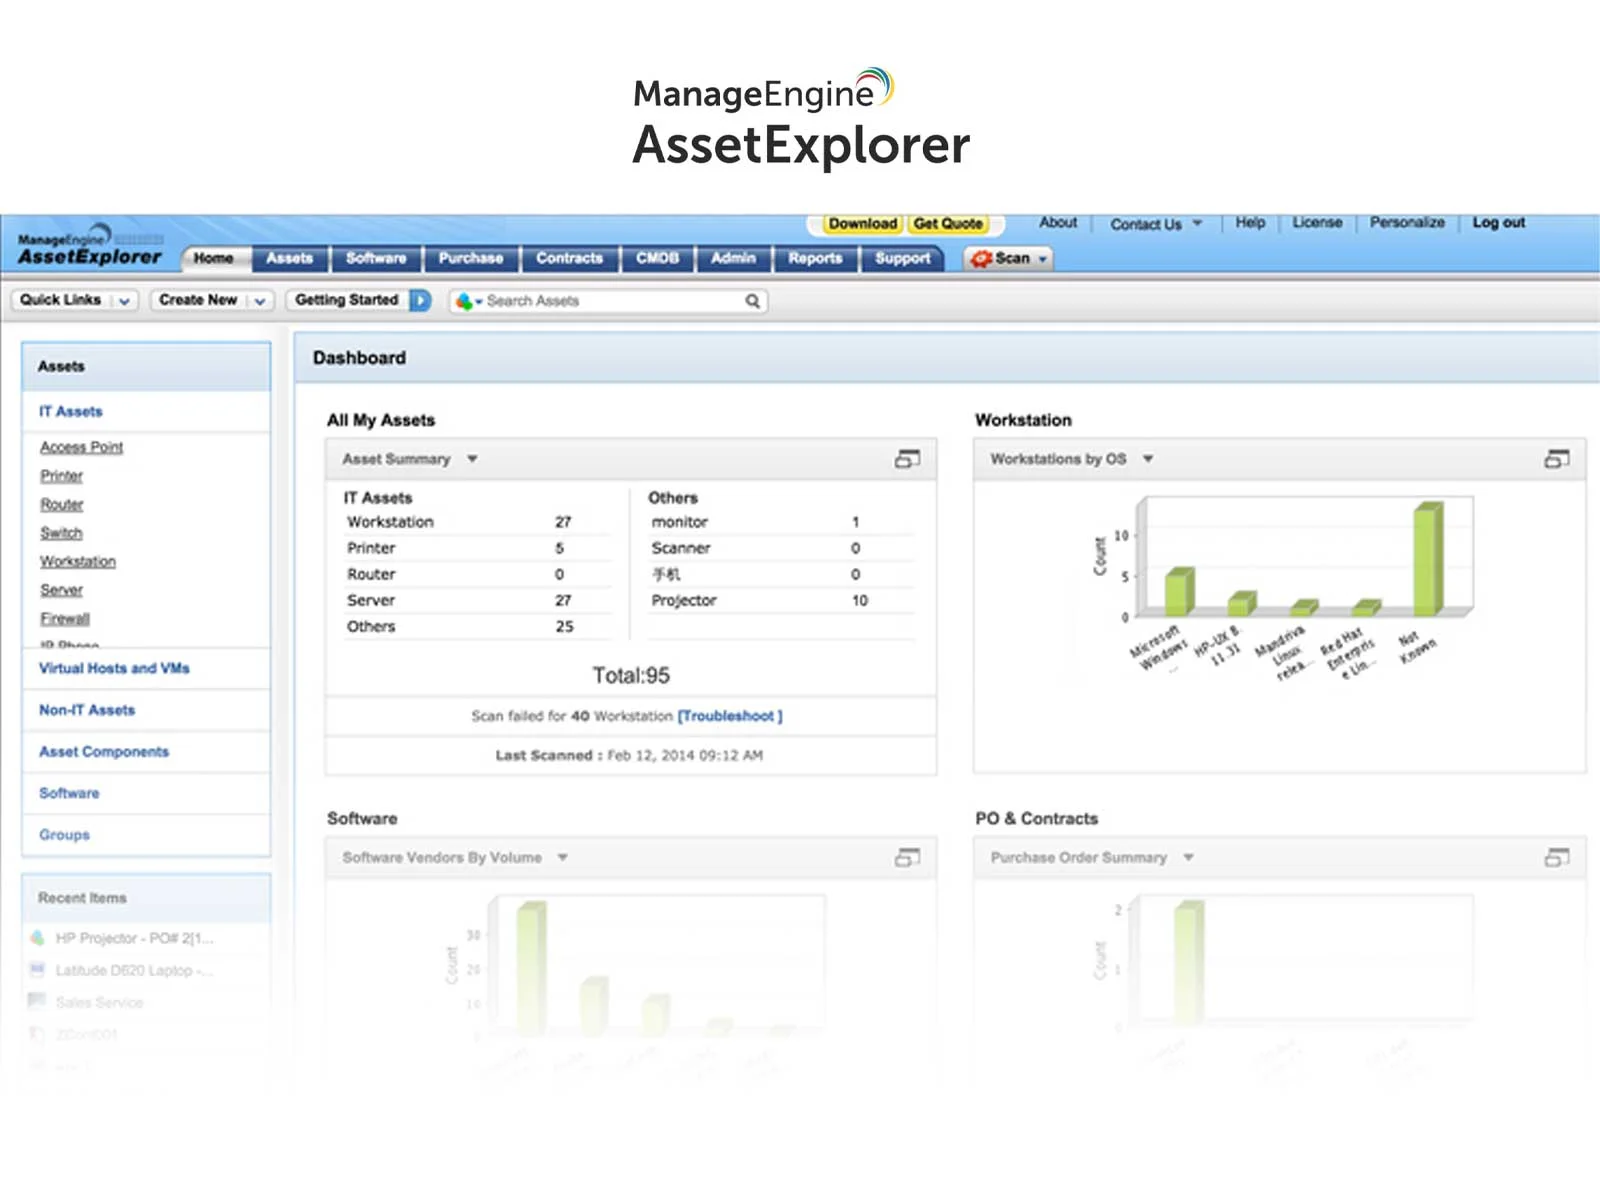
\includegraphics[width=\linewidth]{Images/C3/ManageEngine.png}
%     \caption{ManageEngine Asset Explorer\\ Nguồn: manageengine.com, truy cập vào ngày 01/05/2025}
% \end{figure}

% \noindent \textbf{Các chức năng chính}
% \begin{itemize}[label=--]
%     \item Quản lý kho lưu trữ phần mềm và phần cứng
%     \item Phát hiện và giám sát tài sản
%     \item Ánh xạ và quản lý cấu hình (CMDB)
%     \item Quản lý hợp đồng và giấy phép
%     \item Báo cáo và phân tích
%     \item Quản lý thời hạn dịch vụ và bảo dưỡng
%     \item Lập kế hoạch mua sắm tài sản
%     \item Theo dõi tuân thủ sử dụng
% \end{itemize}
% \textbf{Ưu điểm}
% \begin{itemize}[label=--]
%     \item Quản lý tài sản toàn diện: Asset Explorer không chỉ giúp quản lý tài sản phần cứng và phần mềm mà còn cung cấp nhiều chức năng như quản lý hợp đồng, giấy phép và theo dõi thời hạn bảo dưỡng.
%     \item Ứng dụng di động: Hỗ trợ quản lý tài sản từ xa, tăng tính linh hoạt.
%     \item Quản lý cấu hình dễ dàng: Cơ sở dữ liệu quản lý cấu hình (CMDB) giúp dễ dàng cấu hình và giám sát tài sản mạng để đảm bảo hiệu suất tối ưu.
% \end{itemize}
% \textbf{Nhược điểm}
% \begin{itemize}[label=--]
%     \item Chi phí cho tính năng truy cập từ xa cao: Add-on truy cập từ xa có thể gây khó khăn cho người dùng có ngân sách hạn chế.
%     \item Độ khó cho người mới: Giao diện và tính năng có thể gây khó khăn cho người mới sử dụng.
% \end{itemize}
% \subsection{ServiceNow IT Asset Management}
% \noindent \textbf{ServiceNow IT Asset Management} \cite{servicenow} là một phần của nền tảng ServiceNow, được ra mắt vào năm 2017. Gói dịch vụ này bao gồm mô-đun CMDB cũng như mô-đun SAM đều tương đối mới. Cho phép người dùng quản lý các bản quyền phần mềm, tài sản phần cứng và khả năng theo dõi vòng đời tài sản. Gói dịch vụ này cung cấp cho cả người dùng không sử dụng gói dịch vụ ITSM (quản lý dịch vụ công nghệ thông tin) của ServiceNow.
% \begin{figure}[H]
%     \centering
%     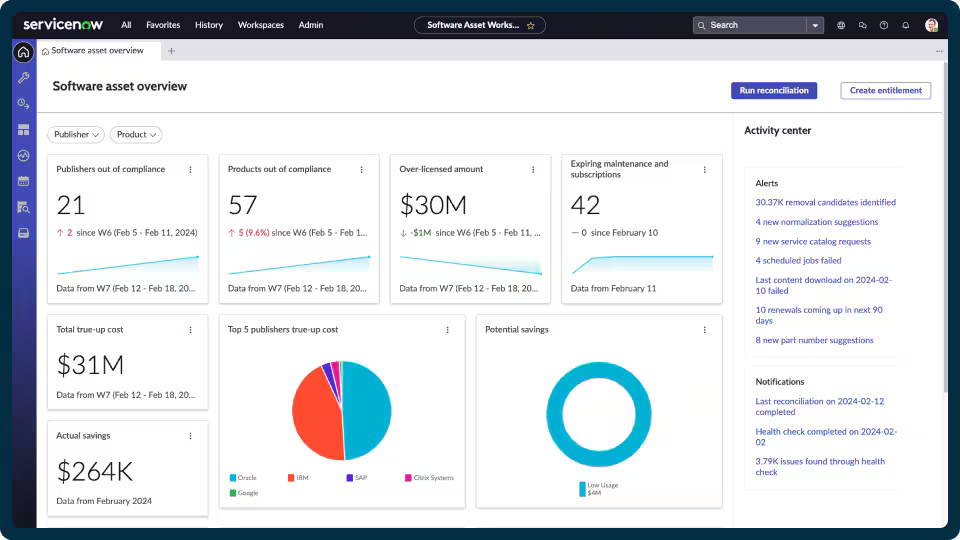
\includegraphics[width=0.8\linewidth]{Images/C3/ServiceNow.png}
%     \vspace{10pt}
%     \caption{ServiceNow IT Asset Management\\ Nguồn: servicenow.com, truy cập vào ngày 01/05/2025}
% \end{figure}

% \noindent \textbf{Các chức năng chính}  
% \begin{itemize}[label=--]
%     \item Quản lý kho lưu trữ phần mềm và phần cứng
%     \item Phát hiện và giám sát tài sản 
%     \item Quản lý tài nguyên đám mây
%     \item Báo cáo và phân tích
%     \item Đăng xuất tài sản CNTT (IT Asset Offboarding)
%     \item Quản lý giấy phép SaaS (Software as a Service)
% \end{itemize}
% \textbf{Ưu điểm}
% \begin{itemize}[label=--]
%     \item Quản lý tài sản tập trung: Tất cả thông tin về tài sản và vòng đời của nó được lưu trữ trong một hệ thống duy nhất.
%     \item Hỗ trợ tích hợp: Có khả năng cập nhật thông tin từ các công cụ khác như AirWatch, SentinelOne.
%     \item Theo dõi và gia hạn giấy phép: Đảm bảo tuân thủ và tránh vi phạm giấy phép.
%     \item Giao diện thân thiện: Hệ thống không chỉ có giao diện thân thiện với người dùng, đảm bảo dễ triển khai mà còn hỗ trợ khách hàng rất tốt, giúp quá trình triển khai trở nên mượt mà.
% \end{itemize}
% \textbf{Nhược điểm}
% \begin{itemize}[label=--]
%     \item Chi phí cao cho doanh nghiệp nhỏ: Phần mềm có thể quá đắt đối với các doanh nghiệp nhỏ.
%     \item Phân quyền phức tạp: Quá trình phân quyền người dùng yêu cầu nhiều bước, dễ gây nhầm lẫn.
%     \item Báo cáo phức tạp: Quá nhiều tùy chọn trong việc tạo báo cáo, đôi khi khiến người dùng khó sử dụng hiệu quả.
%     \item Hiệu suất thấp: Vì có rất nhiều tính năng nên cần dùng nhiều tài nguyên để vận hành, đôi khi hệ thống sẽ phản hồi chậm, làm giảm hiệu  suất.
% \end{itemize}
% \subsection{InvGate Insight}
% \noindent \textbf{InvGate Insight}\cite{invgate} cung cấp cho khách hàng các công cụ để tạo một kho lưu trữ thống nhất cho tất cả tài sản CNTT được kết nối với mạng (bao gồm tài sản ảo, vật lý và trên đám mây) trên cùng một nền tảng. Được nhắm đến các tổ chức vừa và lớn nhưng cũng phù hợp với các công ty nhỏ hơn, Insight cung cấp cái nhìn toàn diện về toàn bộ hệ thống CNTT với cấu hình dễ dàng bằng No-Code/Low-Code mà không cần tích hợp đắt tiền – giảm đáng kể Tổng Chi Phí Sở Hữu (TCO). 
% \begin{figure}[H]
%     \centering
%     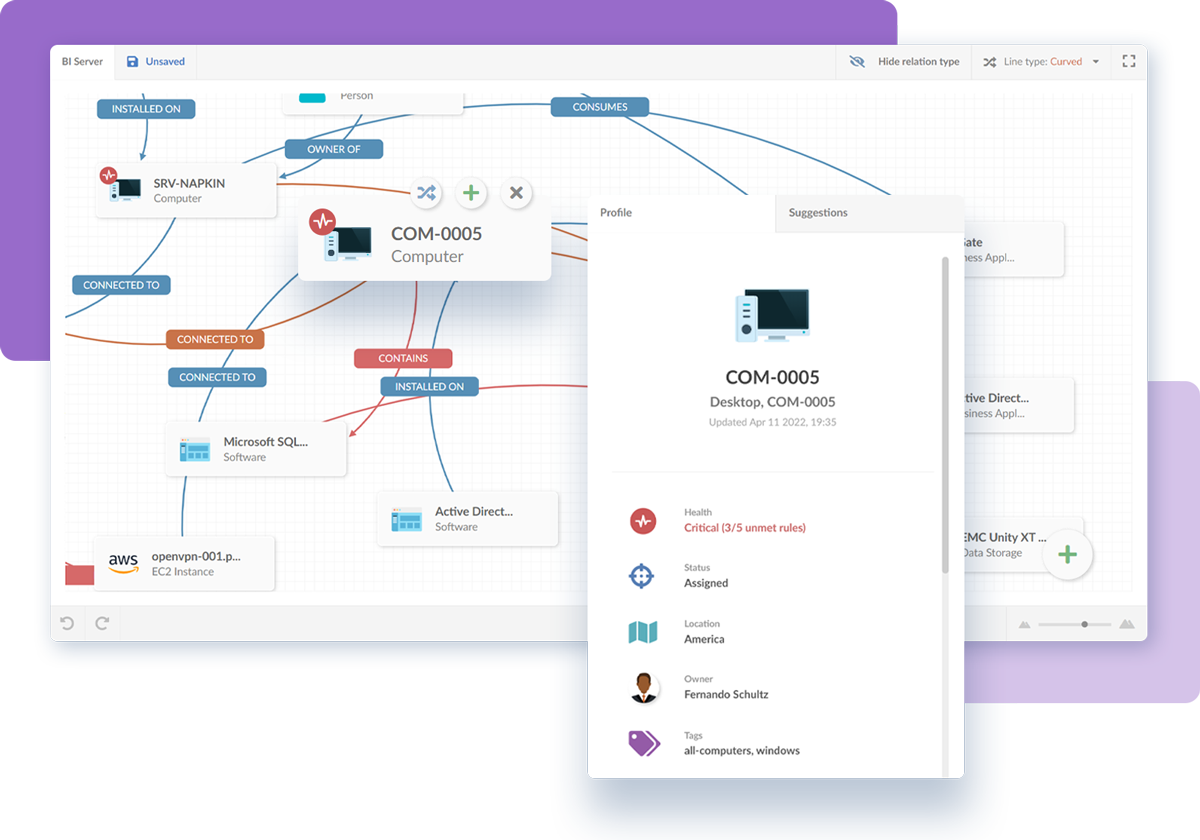
\includegraphics[width=\linewidth]{Images/C3/InvGate_Insight.png}
%     \caption{InvGate Insight\\ Nguồn: invgate.com, truy cập vào ngày 01/05/2025}
% \end{figure}

% \noindent \textbf{Các tính năng chính}
% \begin{itemize}[label=--]
%     \item Quản lý kho lưu trữ phần mềm và phần cứng
%     \item Tự động hóa các quy trình quản lý tài sản
%     \item Cơ sở dữ liệu quản lý cấu hình (CMDB)
%     \item Quản lý tuân thủ an ninh CNTT
%     \item Phát hiện và giám sát tài sản
%     \item Đo lường phần mềm
%     \item Điều khiển từ xa
%     \item Quản lý tài chính CNTT
% \end{itemize}
% \textbf{Ưu điểm}
% \begin{itemize}[label=--]
%     \item Tối ưu hóa cho việc quản lý giấy phép và hợp đồng.
%     \item Được thiết kế để hoạt động liền mách với InvGate Service Desk.
%     \item Tối ưu hóa để giúp tổ chức giảm chi phí, quản lý tuân thủ và rủi ro hiệu quả hơn, cũng như hỗ trợ ra quyết định tốt hơn.
% \end{itemize}
% \textbf{Nhược điểm}
% \begin{itemize}[label=--]
%     \item Hạn chế trong tùy chỉnh: Mặc dù hỗ trợ No-Code/Low-Code, một số chức năng phức tạp hơn vẫn có thể yêu cầu kiến thức kỹ thuật hoặc hỗ trợ từ đội ngũ chuyên gia.
%     \item Không phù hợp với môi trường phi mạng: Giải pháp này tập trung vào tài sản kết nối mạng, do đó có thể không hỗ trợ tốt cho những tổ chức có nhiều tài sản CNTT không được kết nối mạng.
%     \item Chi phí triển khai: Dù không cần tích hợp phức tạp, chi phí cấp phép và duy trì cho các tổ chức nhỏ hoặc rất nhỏ có thể vẫn khá cao.
%     \item Giới hạn tính năng tích hợp bên thứ ba: Có thể không tích hợp tốt với tất cả các công cụ hoặc nền tảng khác mà tổ chức đang sử dụng.
% \end{itemize}
% \subsection{Asset Panda}
% \noindent \textbf{Asset Panda} \cite{assetpanda} là một nền tảng theo dõi tài sản dựa trên đám mây, linh hoạt đáp ứng nhu cầu Quản lý Tài sản cụ thể, chủ yếu hướng đến các doanh nghiệp vừa và nhỏ.
% \begin{figure}[H]
%     \centering
%     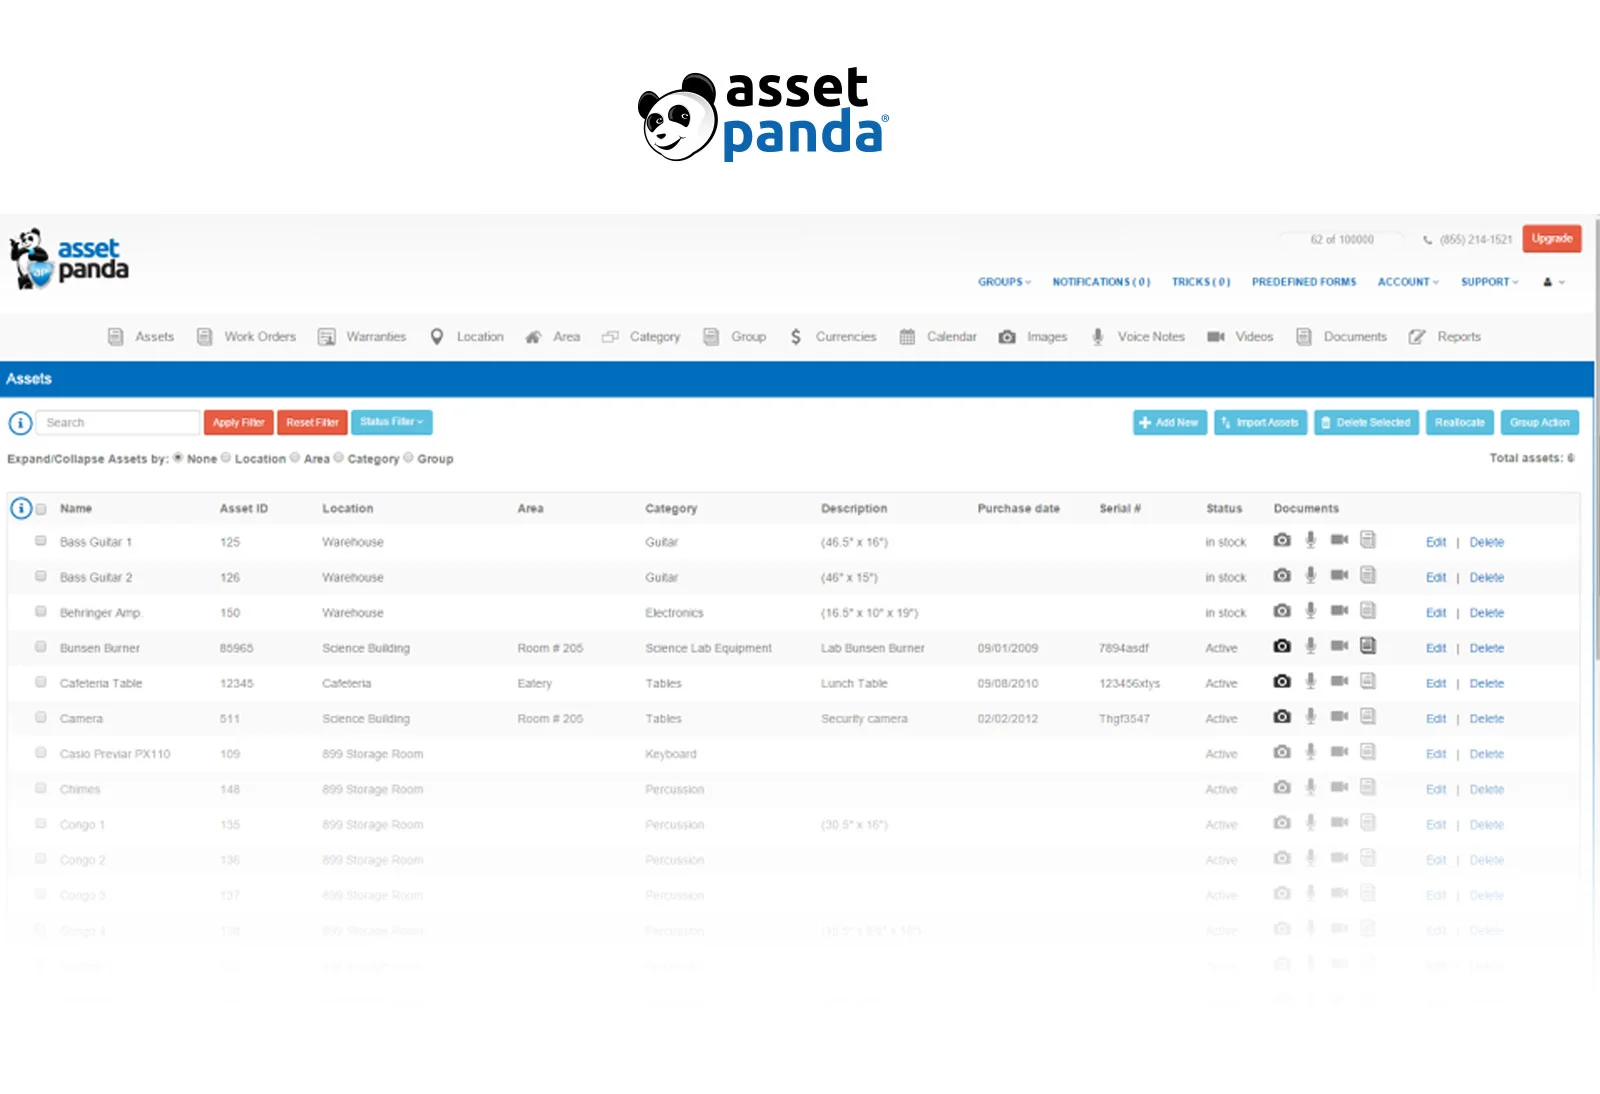
\includegraphics[width=\linewidth]{Images/C3/Asset_Panda.png}
%     \caption{Asset Panda\\ Nguồn: assetpanda.com, truy cập vào ngày 01/05/2025}
% \end{figure}

% \noindent \textbf{Các chức năng chính}
% \begin{itemize}[label=--]
%     \item Ứng dụng di động để cập nhật và theo dõi dữ liệu tài sản CNTT
%     \item Cảnh báo và thông báo về yêu cầu sửa chữa và các sự kiện khác
%     \item Theo dõi toàn bộ vòng đời của tài sản
% \end{itemize}
% \textbf{Ưu điểm}
% \begin{itemize}[label=--]
%     \item Giao diện đơn giản và dễ sử dụng.
%     \item Thông báo và cảnh báo sự kiện tài sản kịp thời.
% \end{itemize}
% \textbf{Nhược điểm}
% \begin{itemize}[label=--]
%     \item Không có chức năng đăng ký người dùng: Điều này có thể gây bất tiện cho việc quản lý người dùng trong hệ thống.
%     \item Không có khả năng theo dõi phần mềm đã cài đặt: Điều này hạn chế việc kiểm soát phần mềm trên các tài sản CNTT.
%     \item Không hỗ trợ phát hiện tài sản theo thời gian thực: Điều này có thể gây khó khăn trong việc theo dõi các tài sản mới hoặc đã thay đổi.
%     \item Báo cáo hạn chế tùy chỉnh.
%     \item Hỗ trợ khách hàng không ổn định.
% \end{itemize} 

% \subsection{Nhận xét chung}
% \noindent Các ứng dụng quản lý tài sản công nghệ thông tin được trình bày bên trên đều có những ưu điểm và nhược điểm riêng \cite{topitam}. Dưới đây là bảng thống kê các tính năng của chúng:
% \begin{table}[h!]
%     \centering
%     \caption{So sánh tính năng giữa các công cụ quản lý tài sản IT}
%     \begin{tabular}{|p{4cm}|p{2.5cm}|p{2.5cm}|p{2.5cm}|p{2.5cm}|}
%         \hline
%         Tính năng & ManageEngine & ServiceNow & InvGate Insight & Asset Panda \\
%         \hline
%         Phát hiện và giám sát tài sản & Có & Có & Có & Có \\
%         \hline
%         Quản lý vòng đời tài sản (Asset Lifecycle) & Có & Có & Có & Có \\
%         \hline
%         Quản lý kho phần cứng và phần mềm & Có & Có & Có & Có \\
%         \hline
%         Báo cáo và phân tích & Có & Có & Có & Có \\
%         \hline
%         Quản lý cấu hình (CMDB) & Có & Có & Có & Có \\
%         \hline
%         Truy cập di động & Add-on & Có & Không & Có \\
%         \hline
%         Tự động phát hiện tài sản & Có & Có & Có & Không \\
%         \hline
%         Tích hợp với hệ thống ITSM & Hạn chế & Toàn diện & Tích hợp liền mạch với InvGate Service Desk & Không \\
%         \hline
%         Quản lý tài nguyên đám mây & Không & Có & Không & Không \\
%         \hline
%         Điều khiển từ xa (Remote Desktop) & Add-on & Có & Có & Không \\
%         \hline
%         Đo lường phần mềm (Software Metering) & Không & Có & Có & Không \\
%         \hline
%         Quản lý tài chính IT & Có & Có & Có & Không \\
%         \hline
%         Quản lý rủi ro và an ninh IT & Có & Có & Có & Không \\
%         \hline
%         Cấu hình No-code/Low-code & Không & Không & Có & Không \\
%         \hline
%         Quản lý giấy phép SaaS & Không & Có & Không & Không \\
%         \hline
%         Giám sát tài sản theo thời gian thực & Có & Có & Có & Không\\
%         \hline
%         Hosting & Đám mây, tại chỗ (Cloud \& On-premise) & Đám mây & Đám mây, tại chỗ (Cloud \& On-premise) & Đám mây\\
%         \hline
%         Thời gian dùng thử & 30 ngày & Không & 30 ngày & 14 ngày\\
%         \hline
%         Chi phí & Bắt đầu từ \$955/năm cho 250 tài sản, lên tới \$11,995/năm cho 10,000 tài sản & Yêu cầu báo giá (Request a quote) & Yêu cầu báo giá (Request a quote) & \$1,500 mỗi năm cho tối đa 500 tài sản\\
%         \hline
%         Chi phí tích hợp & Yêu cầu báo giá & Yêu cầu báo giá & API miễn phí và tích hợp nội bộ & Yêu cầu báo giá \\
%         \hline
%     \end{tabular}    
    
%     \label{table:comparison}
% \end{table}
% \vspace{1em}
% \begin{itemize}[label=--]
%     \item ManageEngine Asset Explorer nổi bật với khả năng quản lý toàn diện tài sản phần cứng và phần mềm, kèm theo tính năng quản lý hợp đồng và giám sát tuân thủ. Tuy nhiên, không hỗ trợ quản lý tài nguyên đám mây và các tính năng nâng cao như SaaS License Management.
%     \item ServiceNow IT Asset Management phù hợp với các tổ chức lớn nhờ tích hợp đầy đủ với ITSM, quản lý tài nguyên đám mây, và quản lý giấy phép SaaS, giúp theo dõi và đảm bảo tuân thủ giấy phép phần mềm.
%     \item InvGate Insight nổi bật với tính năng cấu hình No-code/Low-code và tích hợp chặt chẽ với InvGate Service Desk. Đây là lựa chọn tối ưu cho các tổ chức muốn tùy biến mà không cần chi phí tích hợp cao.
%     \item Asset Panda tập trung vào việc theo dõi tài sản qua di động, nhưng thiếu các tính năng nâng cao như giám sát thời gian thực và quản lý phần mềm SaaS.
% \end{itemize}
% \subsection{Kết chương}
% \noindent Tùy thuộc vào ngân sách, quy mô và yêu cầu cụ thể, sự lựa chọn giữa các hệ thống này này phụ thuộc vào ưu tiên cụ thể của người sử dụng. Nhưng nhìn chung, các hệ thống trên đều có giá rất cao cũng như số lượng dùng thử hạn chế. Thêm vào đó mỗi hệ thống sẽ có một thiên hướng cụ thể về phát hiện hay quản lý tài sản. Ví dụ như Asset Panda tập trung mạnh vào việc quản lý tài sản hay InvGate Insight nổi bật với việc kết hợp phát hiện tài sản mạnh mẽ và phân tích trực quan để giúp đưa ra quyết định quản lý tài sản hiệu quả hơn. Vì lý do như thế, nhóm sẽ hiện thực lại một hệ thống phát hiện và quản lý tài sản CNTT tích hợp cả hai chức năng với giá thành thấp hơn. Quan trọng hơn hết, nhóm tập trung vào tính năng giám sát tài sản thời gian thực.

